\documentclass[tikz]{standalone}

% tikz
\usepackage{tikz, pgfplots}
% i wish external worked but idk it sucks
%\usetikzlibrary{external}
%\tikzexternalize[prefix=figures/]

% for function graph
\usetikzlibrary{positioning}
\usetikzlibrary{shapes.geometric}
\usetikzlibrary{positioning}
\tikzset{
dot/.style = {circle, fill=#1, minimum size=5pt,
              inner sep=0pt, outer sep=0pt},
dot/.default = black % size of the circle diameter
}

 % for braces
\usetikzlibrary{decorations.pathreplacing}
% for hashing area
\usetikzlibrary{patterns}
% tableaux var, signe
% source https://www.sqlpac.com/fr/documents/latex-package-tkz-tab-tikz-tableaux-de-signes-et-de-variations-de-fonctions.html
\usepackage{tkz-tab}
%%%%%%%%%%%%%%%%%%%%%%%%%%%%%%
% SELF MADE COLORS
%%%%%%%%%%%%%%%%%%%%%%%%%%%%%%


\definecolor{myg}{RGB}{56, 140, 70}
\definecolor{myb}{RGB}{45, 111, 177}
\definecolor{myr}{RGB}{199, 68, 64}
\definecolor{mytheorembg}{HTML}{F2F2F9}
\definecolor{mytheoremfr}{HTML}{00007B}
\definecolor{mylenmabg}{HTML}{FFFAF8}
\definecolor{mylenmafr}{HTML}{983b0f}
\definecolor{mypropbg}{HTML}{f2fbfc}
\definecolor{mypropfr}{HTML}{191971}
\definecolor{myexamplebg}{HTML}{F2FBF8}
\definecolor{myexamplefr}{HTML}{88D6D1}
\definecolor{myexampleti}{HTML}{2A7F7F}
\definecolor{mydefinitbg}{HTML}{E5E5FF}
\definecolor{mydefinitfr}{HTML}{3F3FA3}
\definecolor{notesgreen}{RGB}{0,162,0}
\definecolor{myp}{RGB}{197, 92, 212}
\definecolor{mygr}{HTML}{2C3338}
\definecolor{myred}{RGB}{127,0,0}
\definecolor{myyellow}{RGB}{169,121,69}
\definecolor{myexercisebg}{HTML}{F2FBF8}
\definecolor{myexercisefg}{HTML}{88D6D1}
\definecolor{doc}{RGB}{0,60,110}

% manim colors because they're beautiful
% https://docs.manim.community/en/stable/reference/manim.utils.color.manim_colors.html

\definecolor{BLACK}{HTML}{000000}\definecolor{BLUE}{HTML}{58C4DD}\definecolor{BLUE_A}{HTML}{C7E9F1}\definecolor{BLUE_B}{HTML}{9CDCEB}\definecolor{BLUE_C}{HTML}{58C4DD}\definecolor{BLUE_D}{HTML}{29ABCA}\definecolor{BLUE_E}{HTML}{236B8E}\definecolor{DARKER_GRAY}{HTML}{222222}\definecolor{DARKER_GREY}{HTML}{222222}\definecolor{DARK_BLUE}{HTML}{236B8E}\definecolor{DARK_BROWN}{HTML}{8B4513}\definecolor{DARK_GRAY}{HTML}{444444}\definecolor{DARK_GREY}{HTML}{444444}\definecolor{GOLD}{HTML}{F0AC5F}\definecolor{GOLD_A}{HTML}{F7C797}\definecolor{GOLD_B}{HTML}{F9B775}\definecolor{GOLD_C}{HTML}{F0AC5F}\definecolor{GOLD_D}{HTML}{E1A158}\definecolor{GOLD_E}{HTML}{C78D46}\definecolor{GRAY}{HTML}{888888}\definecolor{GRAY_A}{HTML}{DDDDDD}\definecolor{GRAY_B}{HTML}{BBBBBB}\definecolor{GRAY_BROWN}{HTML}{736357}\definecolor{GRAY_C}{HTML}{888888}\definecolor{GRAY_D}{HTML}{444444}\definecolor{GRAY_E}{HTML}{222222}\definecolor{GREEN}{HTML}{83C167}\definecolor{GREEN_A}{HTML}{C9E2AE}\definecolor{GREEN_B}{HTML}{A6CF8C}\definecolor{GREEN_C}{HTML}{83C167}\definecolor{GREEN_D}{HTML}{77B05D}\definecolor{GREEN_E}{HTML}{699C52}\definecolor{GREY}{HTML}{888888}\definecolor{GREY_A}{HTML}{DDDDDD}\definecolor{GREY_B}{HTML}{BBBBBB}\definecolor{GREY_BROWN}{HTML}{736357}\definecolor{GREY_C}{HTML}{888888}\definecolor{GREY_D}{HTML}{444444}\definecolor{GREY_E}{HTML}{222222}\definecolor{LIGHTER_GRAY}{HTML}{DDDDDD}\definecolor{LIGHTER_GREY}{HTML}{DDDDDD}\definecolor{LIGHT_BROWN}{HTML}{CD853F}\definecolor{LIGHT_GRAY}{HTML}{BBBBBB}\definecolor{LIGHT_GREY}{HTML}{BBBBBB}\definecolor{LIGHT_PINK}{HTML}{DC75CD}\definecolor{LOGO_BLACK}{HTML}{343434}\definecolor{LOGO_BLUE}{HTML}{525893}\definecolor{LOGO_GREEN}{HTML}{87C2A5}\definecolor{LOGO_RED}{HTML}{E07A5F}\definecolor{LOGO_WHITE}{HTML}{ECE7E2}\definecolor{MAROON}{HTML}{C55F73}\definecolor{MAROON_A}{HTML}{ECABC1}\definecolor{MAROON_B}{HTML}{EC92AB}\definecolor{MAROON_C}{HTML}{C55F73}\definecolor{MAROON_D}{HTML}{A24D61}\definecolor{MAROON_E}{HTML}{94424F}\definecolor{ORANGE}{HTML}{FF862F}\definecolor{PINK}{HTML}{D147BD}\definecolor{PURE_BLUE}{HTML}{0000FF}\definecolor{PURE_GREEN}{HTML}{00FF00}\definecolor{PURE_RED}{HTML}{FF0000}\definecolor{PURPLE}{HTML}{9A72AC}\definecolor{PURPLE_A}{HTML}{CAA3E8}\definecolor{PURPLE_B}{HTML}{B189C6}\definecolor{PURPLE_C}{HTML}{9A72AC}\definecolor{PURPLE_D}{HTML}{715582}\definecolor{PURPLE_E}{HTML}{644172}\definecolor{RED}{HTML}{FC6255}\definecolor{RED_A}{HTML}{F7A1A3}\definecolor{RED_B}{HTML}{FF8080}\definecolor{RED_C}{HTML}{FC6255}\definecolor{RED_D}{HTML}{E65A4C}\definecolor{RED_E}{HTML}{CF5044}\definecolor{TEAL}{HTML}{5CD0B3}\definecolor{TEAL_A}{HTML}{ACEAD7}\definecolor{TEAL_B}{HTML}{76DDC0}\definecolor{TEAL_C}{HTML}{5CD0B3}\definecolor{TEAL_D}{HTML}{55C1A7}\definecolor{TEAL_E}{HTML}{49A88F}\definecolor{WHITE}{HTML}{FFFFFF}\definecolor{YELLOW}{HTML}{FFFF00}\definecolor{YELLOW_A}{HTML}{FFF1B6}\definecolor{YELLOW_B}{HTML}{FFEA94}\definecolor{YELLOW_C}{HTML}{FFFF00}\definecolor{YELLOW_D}{HTML}{F4D345}\definecolor{YELLOW_E}{HTML}{E8C11C}

% Schwartz
\renewcommand{\S}{\mathcal{S}} % \S est le signe paragraphe normalement

% corps
\newcommand{\C}{\mathcal{C}}
\newcommand{\R}{\mathbb{R}}
\newcommand{\Rnn}{\mathbb{R}^{2n}}
\newcommand{\Z}{\mathbb{Z}}
\newcommand{\N}{\mathbb{N}}
\newcommand{\Q}{\mathbb{Q}}

% domain
\newcommand{\D}{\mathcal{D}}

% order notations
\renewcommand{\O}{\mathcal{O}}

% japanese bracket
\newcommand{\japb}[1]{\langle #1 \rangle}

% arrows over partial derivatives
\newcommand{\lp}{\overleftarrow{\partial}}
\newcommand{\rp}{\overrightarrow{\partial}}

% quantization
\newcommand{\h}{\hbar}
\newcommand{\Opht}{\textrm{Op}_{\h}^{t}}
\newcommand{\Op}[2][\hbar]{\textrm{Op}_{#1}^{#2}}

% omega functions
\newcommand{\omegap}[2][\rho_0]{\omega(\partial_{#1},\partial_{#2})}
\newcommand{\omegar}[2][\rho_0]{\omega(#1,#2)}

\begin{document}
%
	% page 1
	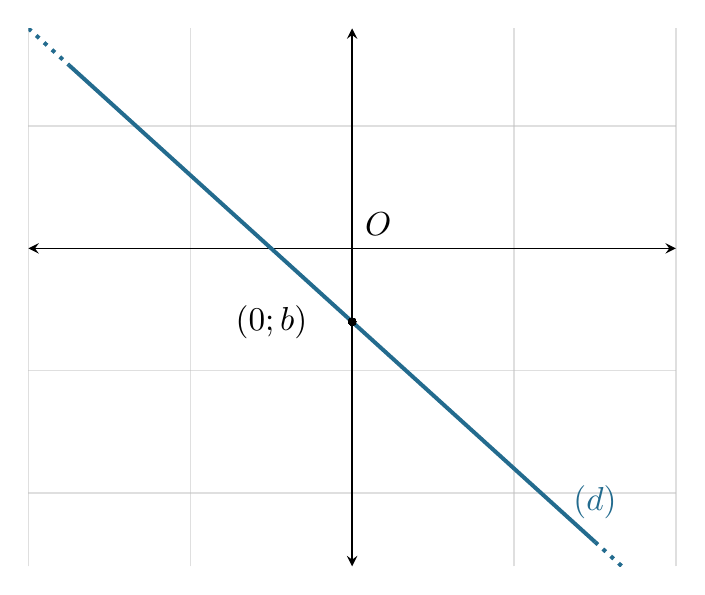
\begin{tikzpicture}[>=stealth, scale=1.2]
	\begin{axis}[xmin = -4, xmax=4, ymin=-13, ymax=9, axis x line=middle, axis y line=middle, axis line style=<->, xlabel={}, ylabel={}, ticks=none, grid=both, grid style = {opacity=.5}]
		\addplot[BLUE_E, very thick, domain =-3.5:3, samples=2] {-3*x-3}  node[above=3pt] {$(d)$};
		\addplot[BLUE_E, very thick, dotted, domain =-4:-3.5, samples=2] {-3*x-3} ;
		\addplot[BLUE_E, very thick, dotted, domain =3:4, samples=2] {-3*x-3};
		\addplot[black, mark=*, mark size = 1] (0,-3) node[left=10pt] {$(0;b)$};
		\addplot[black, very thick] (0,0) node[above right] {$O$};
	\end{axis}
	\end{tikzpicture}
	% page 2
	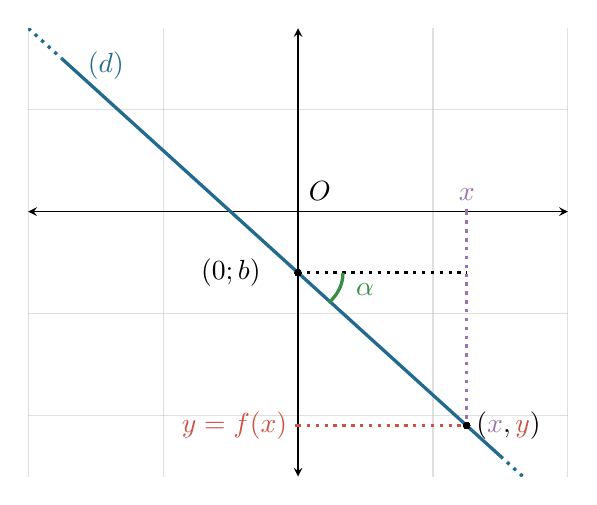
\begin{tikzpicture}[>=stealth, scale=1]
	\begin{axis}[xmin = -4, xmax=4, ymin=-13, ymax=9, axis x line=middle, axis y line=middle, axis line style=<->, xlabel={}, ylabel={}, ticks=none, grid=both, grid style = {opacity=.5}]]
		\addplot[BLUE_E, very thick, domain =-3.5:3, samples=2] {-3*x-3}  node[above=3pt, pos=.1] {$(d)$};
		\addplot[BLUE_E, very thick, dotted, domain =-4:-3.5, samples=2] {-3*x-3} ;
		\addplot[BLUE_E, very thick, dotted, domain =3:4, samples=2] {-3*x-3};
		\addplot[black, mark=*, mark size = 1] (0,-3) node[left=10pt] {$(0;b)$};
		\addplot[black, very thick] (0,0) node[above right] {$O$};
		
		% (x,y)
		\addplot[PURPLE, very thick, mark=|, mark size = 1] (2.5,0) node[above] {$\color{PURPLE} x$};
		\addplot[RED_E, very thick, mark=-, mark size = 1] (0,-10.5) node[left] {$\color{RED_E} y=f(x)$};
		\draw[PURPLE, dotted, very thick] (axis cs:2.5, 0) -- (axis cs:2.5, -10.5);
		\addplot[RED_E, dotted, very thick, domain = 0:2.5, samples=2] {-10.5};
		
		\addplot[black, mark=*, mark size = 1] (2.5,-10.5) node[right] {$({\color{PURPLE} x},{\color{RED_E} y})$};
		
		\addplot[black, dotted, very thick, domain = 0:2.5, samples=2] {-3};
		
		% alpha
		\addplot[myg,very thick,domain=.455:2/3, samples = 30] {(-3-sqrt(4-(x*3)^2))} ;
		\addplot[myg, very thick] (.7,-3) node[below right] {$\alpha$};
	\end{axis}
	\end{tikzpicture}
	% page 3
	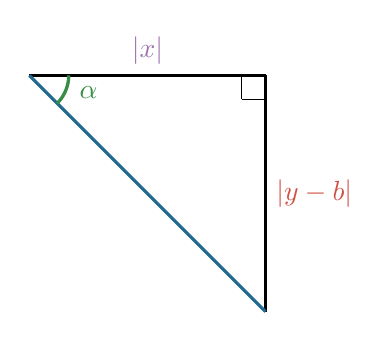
\begin{tikzpicture}[scale=1]
		\draw[-, very thick, black] (0,0) -- (3,0) node[midway, above] {$\color{PURPLE} |x|$};
		\draw[-, very thick, black] (3,0) -- (3,-3) node [midway, right] {$\color{RED_E} |y-b|$};
		\draw[-, very thick, BLUE_E] (3,-3) -- (0,0);
		
		% angle droit
		\draw[-, black] (2.7,0)-- (2.7, -.3);
		\draw[-, black] (2.7, -.3)-- (3, -.3);
		
		% angle
		\draw [myg,very thick,domain=-45:0] plot ({.5*cos(\x)}, {.5*sin(\x)})
		node[below right] {$\color{myg}\alpha$};
	\end{tikzpicture}
	% page 4
	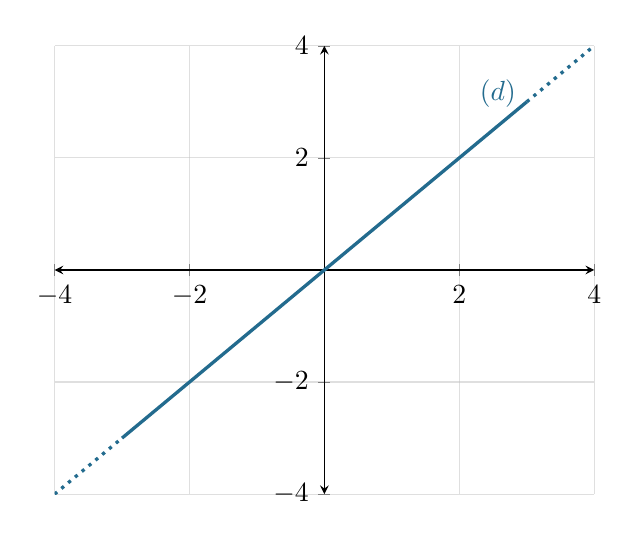
\begin{tikzpicture}[>=stealth, scale=1]
	\begin{axis}[xmin = -4, xmax=4, ymin=-4, ymax=4, axis x line=middle, axis y line=middle, axis line style=<->, xlabel={}, ylabel={}, grid=both, grid style = {opacity=.5}]]
	
		\addplot[BLUE_E, very thick, domain =-3:3, samples=2] {x}  node[above=3pt, left] {$(d)$};
		\addplot[BLUE_E, very thick, dotted, domain =-4:-3, samples=2] {x} ;
		\addplot[BLUE_E, very thick, dotted, domain =3:4, samples=2] {x};
	
		
	\end{axis}
	\end{tikzpicture}
	% page 5
		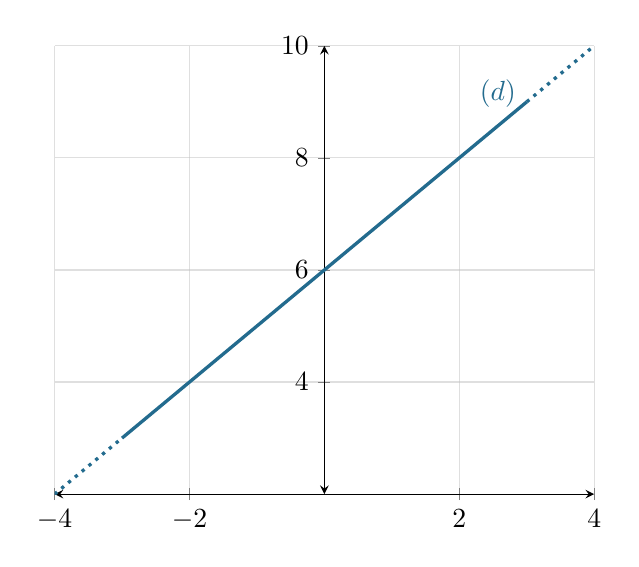
\begin{tikzpicture}[>=stealth, scale=1]
		\begin{axis}[xmin = -4, xmax=4, ymin=2, ymax=10, axis x line=middle, axis y line=middle, axis line style=<->, xlabel={}, ylabel={}, grid=both, grid style = {opacity=.5}]]
		
			\addplot[BLUE_E, very thick, domain =-3:3, samples=2] {x+6}  node[above=3pt, left] {$(d)$};
			\addplot[BLUE_E, very thick, dotted, domain =-4:-3, samples=2] {x+6} ;
			\addplot[BLUE_E, very thick, dotted, domain =3:4, samples=2] {x+6};
		
			
		\end{axis}
	\end{tikzpicture}
	% page 6
	\begin{tikzpicture}[>=stealth, scale=1]
		\begin{axis}[xmin = -4, xmax=4, ymin=1, ymax=4, axis x line=middle, axis y line=middle, axis line style=<->, xlabel={}, ylabel={}, grid=both, grid style = {opacity=.5}]]
		
			\addplot[BLUE_E, very thick, domain =-3:3, samples=2] {2.2}  node[above=3pt] {$(d)$};
			\addplot[BLUE_E, very thick, dotted, domain =-4:-3, samples=2] {2.2} ;
			\addplot[BLUE_E, very thick, dotted, domain =3:4, samples=2] {2.2};
			
		\end{axis}
	\end{tikzpicture}
	% page 7
	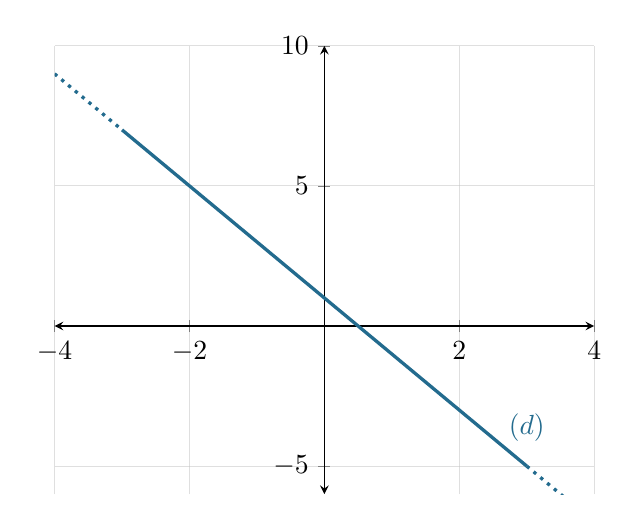
\begin{tikzpicture}[>=stealth, scale=1]
		\begin{axis}[xmin = -4, xmax=4, ymin=-6, ymax=10, axis x line=middle, axis y line=middle, axis line style=<->, xlabel={}, ylabel={}, grid=both, grid style = {opacity=.5}]]
		
			\addplot[BLUE_E, very thick, domain =-3:3, samples=2] {1-2*x}  node[above=5pt] {$(d)$};
			\addplot[BLUE_E, very thick, dotted, domain =-4:-3, samples=2] {1-2*x} ;
			\addplot[BLUE_E, very thick, dotted, domain =3:4, samples=2] {1-2*x};
			
		\end{axis}
	\end{tikzpicture}
	% page 8
	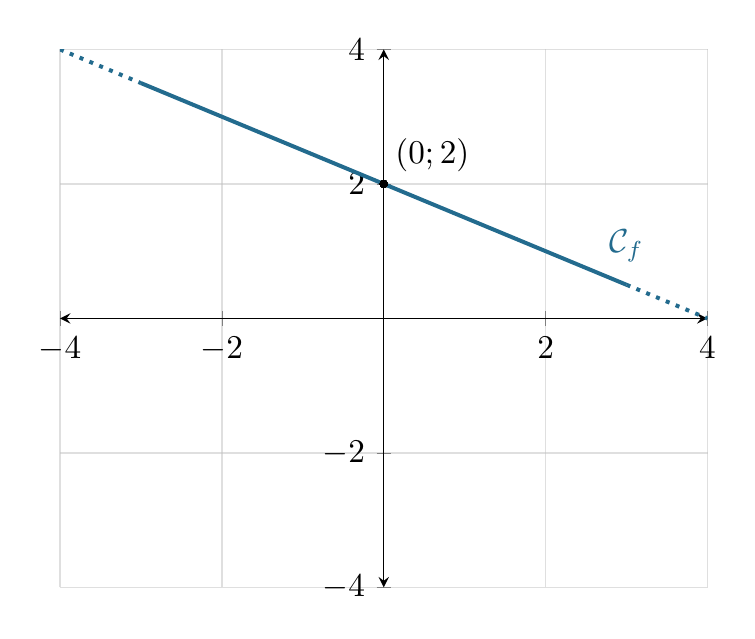
\begin{tikzpicture}[>=stealth, scale=1.2]
	\begin{axis}[xmin = -4, xmax=4, ymin=-4, ymax=4, axis x line=middle, axis y line=middle, axis line style=<->, xlabel={}, ylabel={}, grid=both, grid style = {opacity=.5}]]
		
		% (d)
		\addplot[BLUE_E, very thick, domain =-3:3, samples=2] {2-.5*x}  node[above=3pt] {$\C_f$};
		\addplot[BLUE_E, very thick, dotted, domain =-4:-3, samples=2] {2-.5*x} ;
		\addplot[BLUE_E, very thick, dotted, domain =3:4, samples=2] {2-.5*x};
		
		% (0,b)
		\addplot[black, mark=*, mark size = 1] (0,2) node[above right] {$(0;2)$};
	\end{axis}
	\end{tikzpicture}
	% page 9
	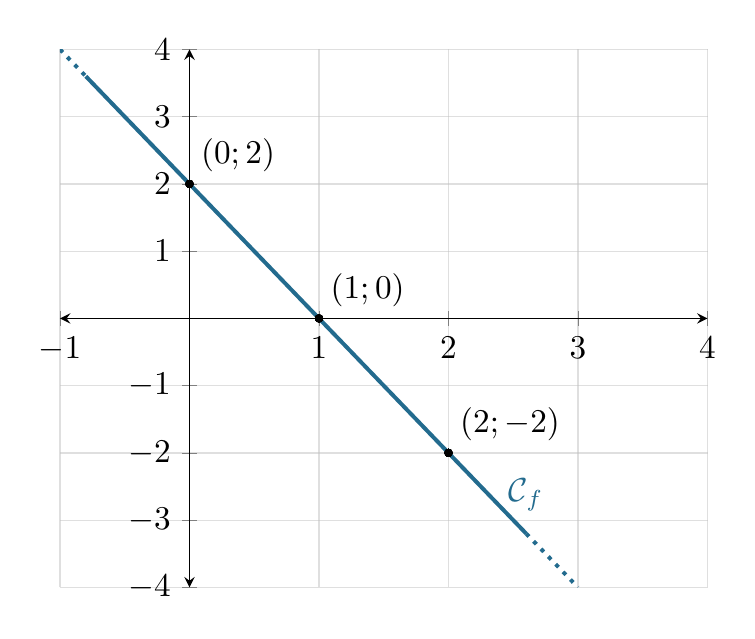
\begin{tikzpicture}[>=stealth, scale=1.2]
	\begin{axis}[xmin = -1, xmax=4, ymin=-4, ymax=4, axis x line=middle, axis y line=middle, axis line style=<->, xlabel={}, ylabel={}, xtick = {-4, -3, ..., 4}, ytick = {-4, -3, ..., 4}, grid=both, grid style = {opacity=.5}]]
		
		% (d)
		\addplot[BLUE_E, very thick, domain =-0.8:2.6, samples=2] {2-2*x}  node[above=3pt] {$\C_f$};
		\addplot[BLUE_E, very thick, dotted, domain =-1:-.8, samples=2] {2-2*x} ;
		\addplot[BLUE_E, very thick, dotted, domain =2.6:3, samples=2] {2-2*x};
		
		% (0,b)
		\addplot[black, mark=*, mark size = 1] (0,2) node[above right] {$(0;2)$};
		
		% (1, b+a)
		\addplot[black, mark=*, mark size = 1] (1,0) node[above right] {$(1;0)$};
		
		% (2, b+2a)
		\addplot[black, mark=*, mark size = 1] (2,-2) node[above right] {$(2;-2)$};
	\end{axis}
	\end{tikzpicture}
	% page 10
	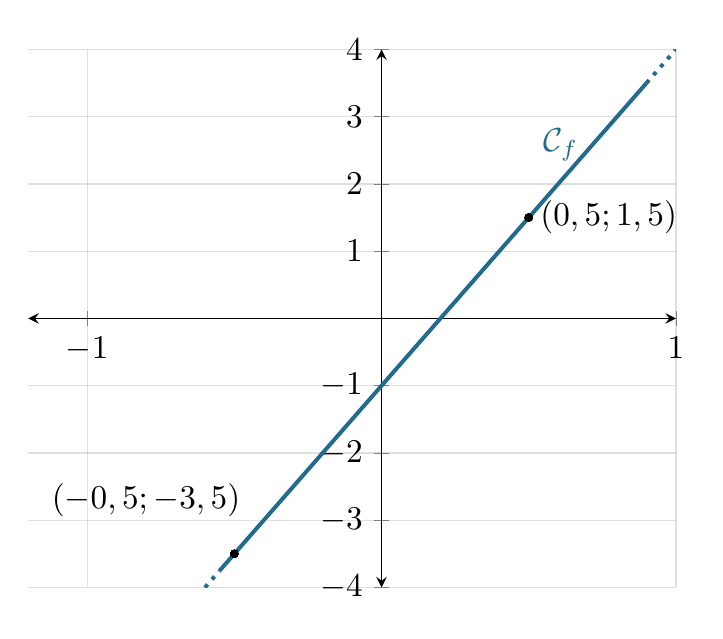
\begin{tikzpicture}[>=stealth, scale=1.2]
	\begin{axis}[xmin = -1.2, xmax=1, ymin=-4, ymax=4, axis x line=middle, axis y line=middle, axis line style=<->, xlabel={}, ylabel={}, xtick = {-4, -3, ..., 4}, ytick = {-4, -3, ..., 4}, grid=both, grid style = {opacity=.5}]]
		
		% (d)
		\addplot[BLUE_E, very thick, domain =-0.55:.9, samples=2] {-1+5*x}  node[pos = .8, above=2pt] {$\C_f$};
		\addplot[BLUE_E, very thick, dotted, domain =-.6:-.55, samples=2] {-1+5*x} ;
		\addplot[BLUE_E, very thick, dotted, domain =.9:1, samples=2] {-1+5*x};
		
		% 2 points
		\addplot[black, mark=*, mark size = 1] (.5,1.5) node[right] {$(0,5 ; 1,5)$};
		\addplot[black, mark=*, mark size = 1] (-.5,-3.5);
		\addplot[black] (-.8,-2.7) node{$(-0,5 ; -3,5)$};
	\end{axis}
	\end{tikzpicture}
	% page 11
	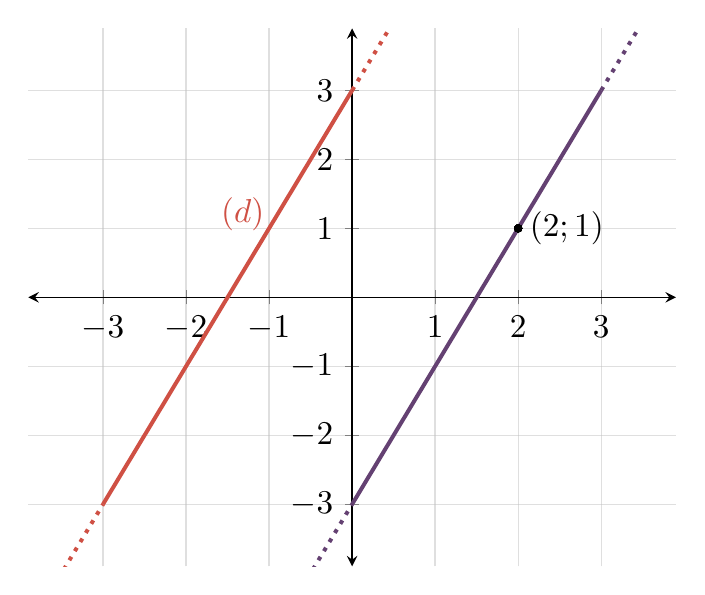
\begin{tikzpicture}[>=stealth, scale=1.2]
		\begin{axis}[xmin = -3.9, xmax=3.9, ymin=-3.9, ymax=3.9, xtick={-3,...,3}, ytick={-3,...,3}, axis x line=middle, axis y line=middle, axis line style=<->, xlabel={}, ylabel={}, grid=both, grid style = {opacity=.5}]]
		
			\addplot[RED_E, very thick, domain =-3:0, samples=2] {2*x+3}  node[left, pos=.7] {$(d)$};
			\addplot[RED_E, dotted, very thick, domain =-4:-3, samples=2] {2*x+3};
			\addplot[RED_E, dotted, very thick, domain =0:1, samples=2] {2*x+3};
			
			\addplot[PURPLE_E, very thick, domain =0:3, samples=2] {2*x-3}  node[above=3pt, left] {};
			\addplot[PURPLE_E, dotted, very thick, domain =-1:0, samples=2] {2*x-3};
			\addplot[PURPLE_E, dotted, very thick, domain =3:4, samples=2] {2*x-3};
		
			\addplot[black, mark=*, mark size = 1] (2,1) node[right] {$(2;1)$};
		
		\end{axis}
	\end{tikzpicture}
%
\end{document}